 \chapter{Architecture}
 \section{Project Workflow}
 The chart below describes the workflow of the project group. The workflow has two independent, parallel flows. The first flow comprises of TVM toolkit and the second flow comprises of the OpenVINO toolkit. First starting with the TVM, we feed the downloaded pre-trained CNN model to the Graph Optimizer of the TVM toolkit. Here it performs graph optimization techniques such as Operator Fusion and Data Layout Formatting. The output is an Intermediate Representation (IR) which contains two files. The first is a JSON file that contains the optimized computational graph and the second file is a PARAM file which contains the quantized weight of the CNN model. This IR is then fed to the Operator Optimizer for further optimization. Operator Optimizer generates an efficient code for each fused operator in the computational graph. This code is then passed to the CodeGen module of the TVM toolkit where it generates the required OpenCL kernel codes. The generated OpenCL kernel codes can be specific to a particular topology or it can be layer specific which can be used in multiple topologies. These generated OpenCL kernel code needs to be customized to be compatible with OpenVINO FPGA plugin. After customization these kernel code are then synthesized for Stratix 10 FPGAs in the Noctua cluster and we create a repository of these bitstreams. We use TVM toolkit solely as a code generator for OpenCL kernel codes.
 
 While the bitstreams repository is being created, we feed the same pre-trained CNN model to the OpenVINO toolkit.The initial stages of the OpenVINO flow is very similar to that of the TVM flow, however there are significant changes in the later stages. Here the CNN model is passed through a Model Optimizer which is similar to Graph Optimizer of the TVM toolkit and employs optimization and quantization techniques. The output is an Intermediate Representation (IR) consisting of an XML file and a BIN file. The XML file contains the optimized computational graph and BIN file contains the quantized weight of the CNN model. This IR is then passed to the Inference Engine of the OpenVINO toolkit. Now the developed OpenVINO FPGA plugin is a part of the Inference Engine. The Inference Engine first parses the IR. Then according to the layer-name or layer-number the FPGA plugin will pick up the corresponding bitstream from the bitstream repository, flash them onto the FPGA and launch the appropriate kernel. The Inference Engine provides a C++ API to an application level program where the inference result can be displayed. Using this API the users can give a single image or batch of images as an input to be classified.
 \begin{figure}[h!]
    \centering
    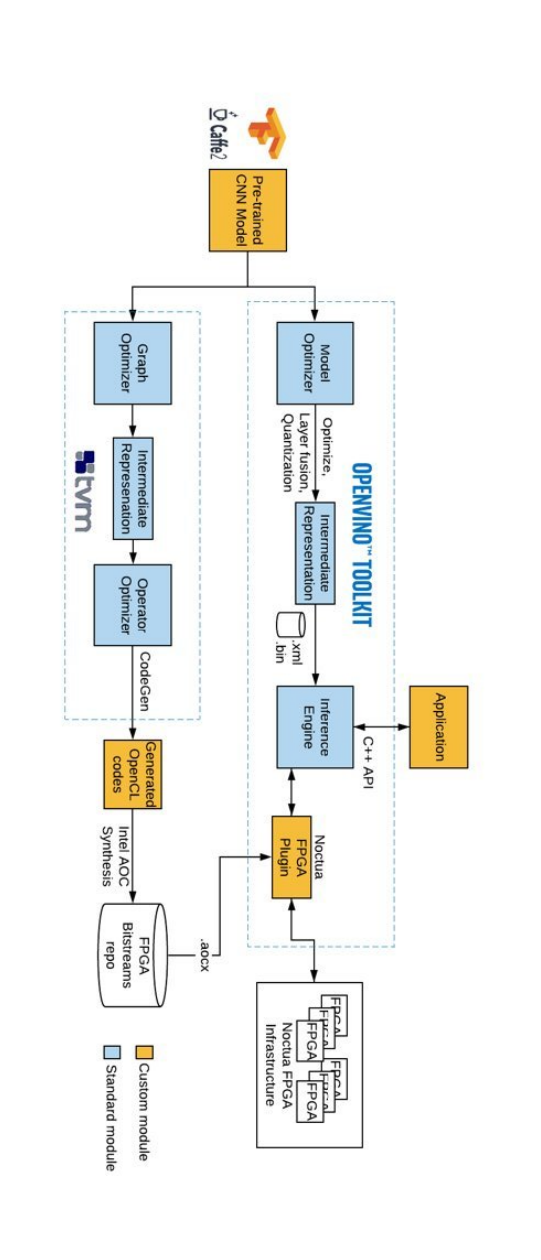
\includegraphics[scale=1]{workflow1.png}
    \caption{OpenVINO Flowchart}
\end{figure}

\begin{figure}[h!]
    \centering
    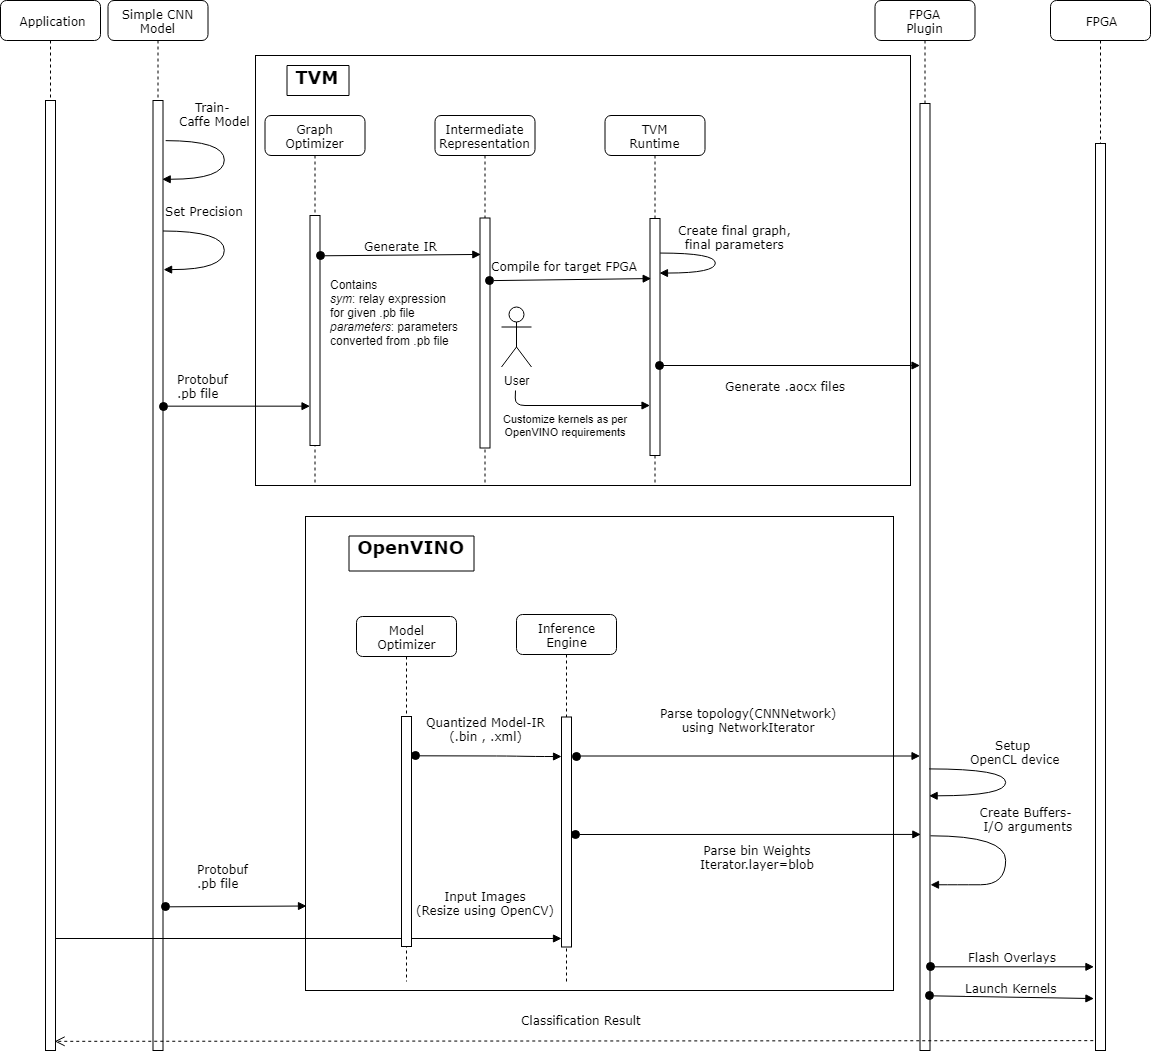
\includegraphics[scale=0.4]{DesignDocument.png}
    \caption{Sequence Diagram of the Project Workflow}
\end{figure}

\section{TVM}
\subsection{Frontend}
\subsection{Codegen}

\section{OpenVino}
\subsection{Inference Engine}
\subsection{Model Optimiser}
\subsection{MPI}

Message Passing Interface (MPI) allows sending data between processes. It’s an open-source library that has standard functions for initializing message-passing functions, assigning a rank to each process and proceeding communication among them via send and receive calls. It provides scalability for FPGA plugin.


Initially, when we invoke launching command we have only one process or one node (Fig. \ref{fig:node}). Each node has two devices (FPGAs), which share global memory. Communication between devices on one node gets through the context and between nodes through sending and receiving calls.

\begin{figure}[!htb]
  \centering
  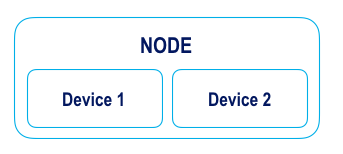
\includegraphics[width=0.4\textwidth,height=0.4\textheight,keepaspectratio]{img/node.png}
  \caption{Image of one node where two devices have access to global memory.}
  \label{fig:node}
\end{figure}
